\section{Estimación de parámetros}

%\subsection{Modelo con una clase}
\subsection{Modelo multiclase con datos sintéticos}

Usando condiciones iniciales, un valor de P... matrices de convarianza... 

\begin{figure}[h]
\centering
\includegraphics[width=0.99\textwidth]{img/resultados/synth/kalman_grouped_allstates_allgroups\parameterstring}
\caption{Resultados obtenidos con Filtro de Kalman Suavizado para el caso sintético.}
\label{synth-all-nohigh}
\end{figure}



\begin{figure}
     \centering
     \begin{subfigure}[b]{\textwidth}
         \centering
         \includegraphics[width=.8\textwidth]{img/resultados/synth/kalman_grouped_E_high1\parameterstring}
         \caption{Clase \(1\).}
     \end{subfigure}
     \hfill
     \begin{subfigure}[b]{\textwidth}
         \centering
         \includegraphics[width=0.8\textwidth]{img/resultados/synth/kalman_grouped_E_high2\parameterstring}
         \caption{Clase \(2\).}
     \end{subfigure}
        \caption{Casos Expuestos, comparando resultados obtenidos con solución real, en valores absolutos y normalizados con respecto a la cantidad de personas por clase.}
        \label{synth-e-comp-high}
\end{figure}

\begin{figure}
     \centering
     \begin{subfigure}[b]{\textwidth}
         \centering
         \includegraphics[width=.99\textwidth]{img/resultados/synth/kalman_grouped_alpha_high1\parameterstring}
         \caption{Clase \(1\).}
     \end{subfigure}
     \hfill
     \begin{subfigure}[b]{\textwidth}
         \centering
         \includegraphics[width=0.99\textwidth]{img/resultados/synth/kalman_grouped_alpha_high2\parameterstring}
         \caption{Clase \(2\).}
     \end{subfigure}
        \caption[Factor sanitario, caso sintético]{Factor sanitario, comparando resultados obtenidos con función de control usada para general los datos, acotando el dominio en el eje \(y\) para mejor apreciación.}
        \label{synth-alpha-comp-high}
\end{figure}


\subsection{Análisis de sensibilidad}


En la práctica los riesgos \(\beta \), las tasas \(\gamma_E\) y \(\gamma_I\), así como las condiciones iniciales serán valores desconocidos. Esta sección estudia el efecto de estos valores en la solución estimada. 

% gamma_e_real = 1/5.1; gamma_i_real = 1/7.2; beta_exterior_real = 1.88; 
Utilizando el caso sintético ya presentado, se estudia el efecto del valor \(\beta_{\text{exterior}}\) y de las condiciones iniciales para factor sanitario \(\alpha\) en los resultados. Los datos fueron generados con \(\gamma_E = 1/5.1 [\text{días}]^{-1}\), \(\gamma_I = 1/7.2 [\text{días}]^{-1}\) y \(\beta_{\text{exterior}} = 1.88\). Para distintos valores de \(\beta_{\text{exterior}}\) y distintas condiciones iniciales para el factor sanitario, se estima el factor sanitario y se compara con el valor de control usado para generar los datos. Los resultados pueden verse en la figura \ref{fig:legend-sensi-b}.

Se observa que tras una cierta cantidad de tiempo (\(t \geq 50\) la condición inicial es irrelevante y todas las soluciones dadas por un mismo \(\beta_{\text{exterior}}\) siguen la misma trayectoria. Al comenzar en una condición inicial demasiado baja, como \(\alpha_0 = 0.15\), se observa una tendencia a sobrecorregir el error, lo que produce una sobreestimación antes de llegar a la trayectoria común.

Se utilizó 


\begin{figure}
\centering
\begin{tabular}{c c}
\begin{subfigure}[b]{0.75\textwidth}
     \centering
     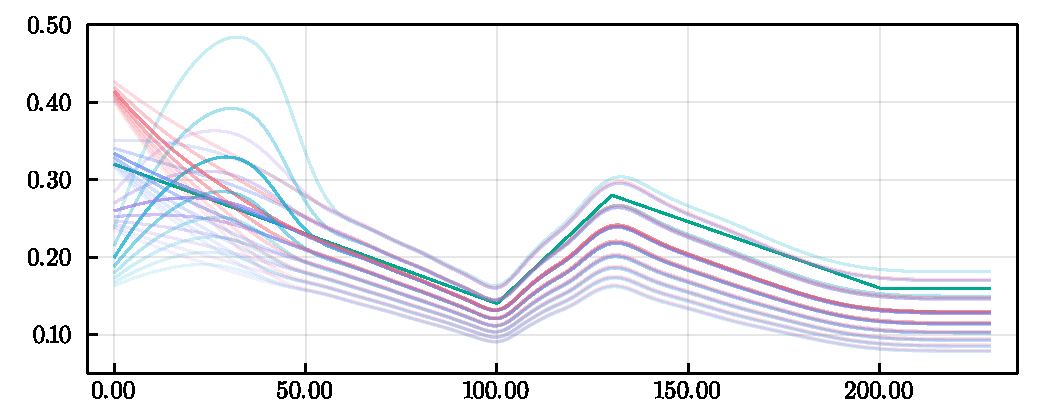
\includegraphics[width=\textwidth]{img/resultados/synth/sensibeta1-2_0-3_3-4_alpha0-15_0-1_0-45high1b2real1-88_gereal0-1961_gireal0-1389_acov0-8_aini0-27675_gcov0-05gamma_e_0-1724_gamma_i_0-1220_beta_2_2-0000.pdf}
     \caption{\(\gamma = 1.3 \)}
\end{subfigure} & \multirow{2}{*}{
\begin{subfigure}[b]{0.15\textwidth}
 \centering
\scalebox{0.5}{
\begin{tikzpicture}
	\begin{pgfonlayer}{nodelayer}
		\node [style=none] (0) at (1, 2) {};
		\node [style=none] (1) at (2.5, 2) {};
		\node [style=none] (2) at (1, 1.5) {};
		\node [style=none] (3) at (2.5, 1.5) {};
		\node [style=none] (4) at (1, 1) {};
		\node [style=none] (5) at (2.5, 1) {};
		\node [style=none] (6) at (1, 0.5) {};
		\node [style=none] (7) at (2.5, 0.5) {};
		\node [style=none] (8) at (3, 2) {$0.15$};
		\node [style=none] (9) at (3, 1.5) {};
		\node [style=none] (10) at (3, 1.5) {};
		\node [style=none] (11) at (3, 1.5) {$0.25$};
		\node [style=none] (12) at (3, 1) {};
		\node [style=none] (13) at (3, 1) {$0.35$};
		\node [style=none] (15) at (3, 0.5) {$0.45$};
		\node [style=none] (17) at (2, 2.5) {Condición inicial $\alpha_0$};
		\node [style=none] (19) at (2, -1.5) {$\beta_{\textrm{ext}}$};
		\node [style=none] (21) at (2, -0.25) {$\beta_{\text{ext}}$ solución real};
		\node [style=none] (22) at (1, -0.75) {};
		\node [style=none] (23) at (2.5, -0.75) {};
		\node [style=none] (24) at (3, -0.75) {};
		\node [style=none] (25) at (3, -0.75) {$1.88$};
		\node [style=none] (26) at (1, -2) {};
		\node [style=none] (27) at (2.5, -2) {};
		\node [style=none] (28) at (1, -2.5) {};
		\node [style=none] (29) at (2.5, -2.5) {};
		\node [style=none] (30) at (1, -3) {};
		\node [style=none] (31) at (2.5, -3) {};
		\node [style=none] (32) at (1, -3.5) {};
		\node [style=none] (33) at (2.5, -3.5) {};
		\node [style=none] (34) at (1, -4) {};
		\node [style=none] (35) at (2.5, -4) {};
		\node [style=none] (36) at (1, -4.5) {};
		\node [style=none] (37) at (2.5, -4.5) {};
		\node [style=none] (38) at (1, -5) {};
		\node [style=none] (39) at (2.5, -5) {};
		\node [style=none] (40) at (1, -5.5) {};
		\node [style=none] (41) at (2.5, -5.5) {};
		\node [style=none] (42) at (3, -2) {$1.2$};
		\node [style=none] (43) at (3, -2.5) {$1.5$};
		\node [style=none] (44) at (3, -3) {$1.8$};
		\node [style=none] (45) at (3, -3.5) {$2.1$};
		\node [style=none] (46) at (3, -4) {$2.4$};
		\node [style=none] (47) at (3, -4.5) {$2.7$};
		\node [style=none] (48) at (3, -5) {$3.0$};
		\node [style=none] (49) at (3, -5.5) {$3.3$};
		\node [style=none] (50) at (0, 3.25) {};
		\node [style=none] (51) at (4, 3.25) {};
		\node [style=none] (52) at (4, -6.25) {};
		\node [style=none] (53) at (0, -6.25) {};
	\end{pgfonlayer}
	\begin{pgfonlayer}{edgelayer}
		\draw [style={a0_1}] (0.center) to (1.center);
		\draw [style={a0_2}] (2.center) to (3.center);
		\draw [style={a0_3}] (4.center) to (5.center);
		\draw [style={a0_4}] (6.center) to (7.center);
		\draw [style=real] (22.center) to (23.center);
		\draw [style=beta1] (26.center) to (27.center);
		\draw [style=beta2] (28.center) to (29.center);
		\draw [style=beta3] (30.center) to (31.center);
		\draw [style=beta4] (32.center) to (33.center);
		\draw [style=beta5] (34.center) to (35.center);
		\draw [style=beta6] (36.center) to (37.center);
		\draw [style=beta7] (38.center) to (39.center);
		\draw [style=beta8] (40.center) to (41.center);
		\draw (50.center) to (51.center);
		\draw (51.center) to (52.center);
		\draw (52.center) to (53.center);
		\draw (53.center) to (50.center);
	\end{pgfonlayer}
\end{tikzpicture}
}
\end{subfigure}} \\
\begin{subfigure}[b]{0.75\textwidth}
     \centering
     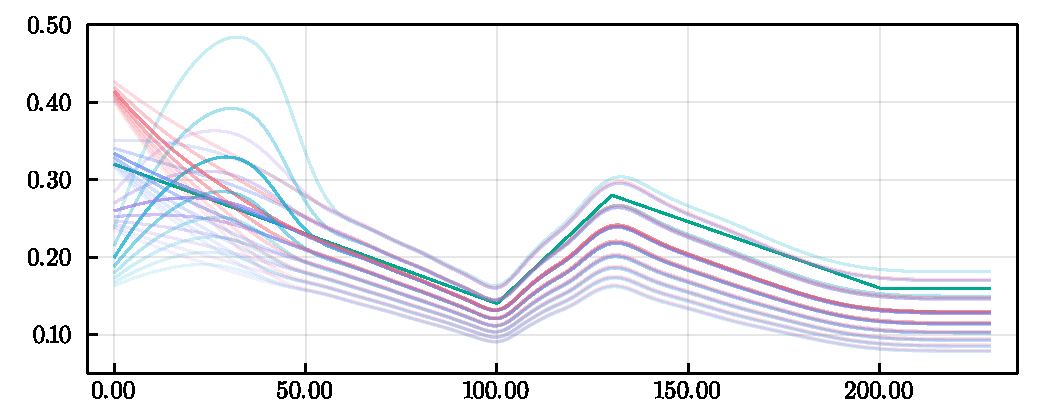
\includegraphics[width=\textwidth]{img/resultados/synth/sensibeta1-2_0-3_3-4_alpha0-15_0-1_0-45high1b2real1-88_gereal0-1961_gireal0-1389_acov0-8_aini0-27675_gcov0-05gamma_e_0-1724_gamma_i_0-1220_beta_2_2-0000.pdf}
     \caption{\(\gamma = 2.1\)}
\end{subfigure} & \\
\end{tabular}
\caption[Sensibilidad ante riesgo exterior y condición inicial del factor sanitario.]{Sensibilidad ante riesgo exterior y condición inicial del factor sanitario. Cada color representa un condición inicial diferente usada en la estimación, mientras que la opacidad de la solución representa la distancia de \(\beta_{\text{exterior}}\) al valor real; a mayor transparencia, más lejano.} \label{fig:legend-sensi-b}
\end{figure}




\subsection{Modelo con datos reales}


\begin{figure}[h]
\centering
\includegraphics[width=0.99\textwidth]{img/resultados/kalman_grouped_allstates_allgroups\parameterstring}
\caption{Resultados obtenidos con Filtro de Kalman Suavizado para el caso real.}
\label{all-nohigh}
\end{figure}



\begin{figure}
     \centering
     \begin{subfigure}[b]{0.47\textwidth}
         \centering
         \includegraphics[width=\textwidth]{img/resultados/kalman_grouped_I_high1\parameterstring}
         \caption{Clase \(1\).}
     \end{subfigure}
     \hfill
     \begin{subfigure}[b]{.47\textwidth}
         \centering
         \includegraphics[width=\textwidth]{img/resultados/kalman_grouped_I_high2\parameterstring}
         \caption{Clase \(2\).}
     \end{subfigure}
     \hfill
     \begin{subfigure}[b]{.47\textwidth}
         \centering
         \includegraphics[width=\textwidth]{img/resultados/kalman_grouped_I_high3\parameterstring}
         \caption{Clase \(3\).}
     \end{subfigure}
     \hfill
     \begin{subfigure}[b]{.47\textwidth}
         \centering
         \includegraphics[width=\textwidth]{img/resultados/kalman_grouped_I_high4\parameterstring}
         \caption{Clase \(4\).}
     \end{subfigure}
     \hfill
     \begin{subfigure}[b]{.47\textwidth}
         \centering
         \includegraphics[width=\textwidth]{img/resultados/kalman_grouped_I_high5\parameterstring}
         \caption{Clase \(5\).}
     \end{subfigure}
     \hfill
     \begin{subfigure}[b]{.47\textwidth}
         \centering
         \includegraphics[width=\textwidth]{img/resultados/kalman_grouped_I_allclass\parameterstring}
         \caption{Todas las clases.}
     \end{subfigure}
        \caption{Cantidad de Infectados estimados a partir de datos reales, en valores absolutos y normalizados con respecto a la cantidad de personas por clase.}
        \label{e-comp-high}
\end{figure}



\begin{figure}
     \centering
     \begin{subfigure}[b]{0.47\textwidth}
         \centering
         \includegraphics[width=\textwidth]{img/resultados/kalman_grouped_S_high1\parameterstring}
         \caption{Clase \(1\).}
     \end{subfigure}
     \hfill
     \begin{subfigure}[b]{.47\textwidth}
         \centering
         \includegraphics[width=\textwidth]{img/resultados/kalman_grouped_S_high2\parameterstring}
         \caption{Clase \(2\).}
     \end{subfigure}
     \hfill
     \begin{subfigure}[b]{.47\textwidth}
         \centering
         \includegraphics[width=\textwidth]{img/resultados/kalman_grouped_S_high3\parameterstring}
         \caption{Clase \(3\).}
     \end{subfigure}
     \hfill
     \begin{subfigure}[b]{.47\textwidth}
         \centering
         \includegraphics[width=\textwidth]{img/resultados/kalman_grouped_S_high4\parameterstring}
         \caption{Clase \(4\).}
     \end{subfigure}
     \hfill
     \begin{subfigure}[b]{.47\textwidth}
         \centering
         \includegraphics[width=\textwidth]{img/resultados/kalman_grouped_S_high5\parameterstring}
         \caption{Clase \(5\).}
     \end{subfigure}
     \hfill
     \begin{subfigure}[b]{.47\textwidth}
         \centering
         \includegraphics[width=\textwidth]{img/resultados/kalman_grouped_S_allclass\parameterstring}
         \caption{Todas las clases.}
     \end{subfigure}
        \caption{Cantidad de Susceptibles estimados a partir de datos reales, en valores absolutos y normalizados con respecto a la cantidad de personas por clase.}
        \label{s-comp-high}
\end{figure}




\begin{figure}
     \centering
     \begin{subfigure}[b]{.99\textwidth}
         \centering
         \includegraphics[width=\textwidth]{img/resultados/kalman_grouped_alpha_allclass\parameterstring}
         \caption{Todas las clases.}
     \end{subfigure}
     \hfill
     \begin{subfigure}[b]{0.47\textwidth}
         \centering
         \includegraphics[width=\textwidth]{img/resultados/kalman_grouped_alpha_high1\parameterstring}
         \caption{Clase \(1\).}
     \end{subfigure}
     \hfill
     \begin{subfigure}[b]{.47\textwidth}
         \centering
         \includegraphics[width=\textwidth]{img/resultados/kalman_grouped_alpha_high2\parameterstring}
         \caption{Clase \(2\).}
     \end{subfigure}
     \hfill
     \begin{subfigure}[b]{.47\textwidth}
         \centering
         \includegraphics[width=\textwidth]{img/resultados/kalman_grouped_alpha_high3\parameterstring}
         \caption{Clase \(3\).}
     \end{subfigure}
     \hfill
     \begin{subfigure}[b]{.47\textwidth}
         \centering
         \includegraphics[width=\textwidth]{img/resultados/kalman_grouped_alpha_high4\parameterstring}
         \caption{Clase \(4\).}
     \end{subfigure}
     \hfill
     \begin{subfigure}[b]{.47\textwidth}
         \centering
         \includegraphics[width=\textwidth]{img/resultados/kalman_grouped_alpha_high5\parameterstring}
         \caption{Clase \(5\).}
     \end{subfigure}
        \caption[Factor sanitario estimado a partir de datos reales.]{Factor sanitario estimado a partir de datos reales. Las líneas grises corresponden a algunas fechas relevantes: (1) 13/may/2020 - Comienzo de la cuarentena total en la RM; (2) 25/oct/2020 - Plesbicito por la nueva constitución; (3) 4/ene/2021 - Comienza a funcionar el pase de vacaciones; (4) 1/feb/2021 - Comienza un plan de vacunación más intensivo (ver visualizador CMM); (5) 26/may/2021 - Un 50\% de la población en la RM tiene la primera dosis de la vacuna.}
        \label{s-comp-high}
\end{figure}


